\newpage\BorderFirstPage
\chapter[~]{Знайомство з програмою для розробки креслень sPlan}
\textbf{Мета роботи} --- ознайомитись з призначенням та основними прийомами роботи в програмі для
розробки креслень схем sPlan, навчитись виконувати креслення простих схем.


\section{Короткі теоретичні відомості}

\textbf{Програма sPlan} --- простий і зручний інструмент для креслення електронних і електричних
схем, вона дозволяє легко переносити символи з бібліотеки елементів на схему і прив'язувати їх до
координатної сітки.

Програма підтримує автоматичну нумерацію елементів, контактів та можливість задання номіналів для
елементів. Також є можливість створювати власні шаблони документів, а також компоненти та
бібліотеки, що дає змогу створювати набори стандартних компонентів і поширювати їх між розробниками.

В функціонал також входить робота з текстовими елементами та таблицями. Також можна згенерувати
перелік використаних компонентів.

Є можливість задавати розмірні лінії, що може бути зручним для схематичного зображення об'єктів.

Один документ в sPlan може мати декілька сторінок різних форматів, що полегшує роботу з
багатосторінковими елементами.

Якщо в документі є повторювані значення, наприклад шифр документу то його можна задати у вигляді
користувацької змінної, і вставляти автоматично. Це може бути також використано при створенні
шаблонних документів.

\newpage
\BorderText
\restoregeometry
\section{Виконання роботи}

\begin{enumerate}[leftmargin=*]
\item З стандартної бібліотеки вибираємо необхідні компоненти і перетягуємо їх на аркуш та
  розміщуємо у потрібному положенні (\ref{fig:lab1:step1}).
  \begin{figure}[!ht]
    \centering 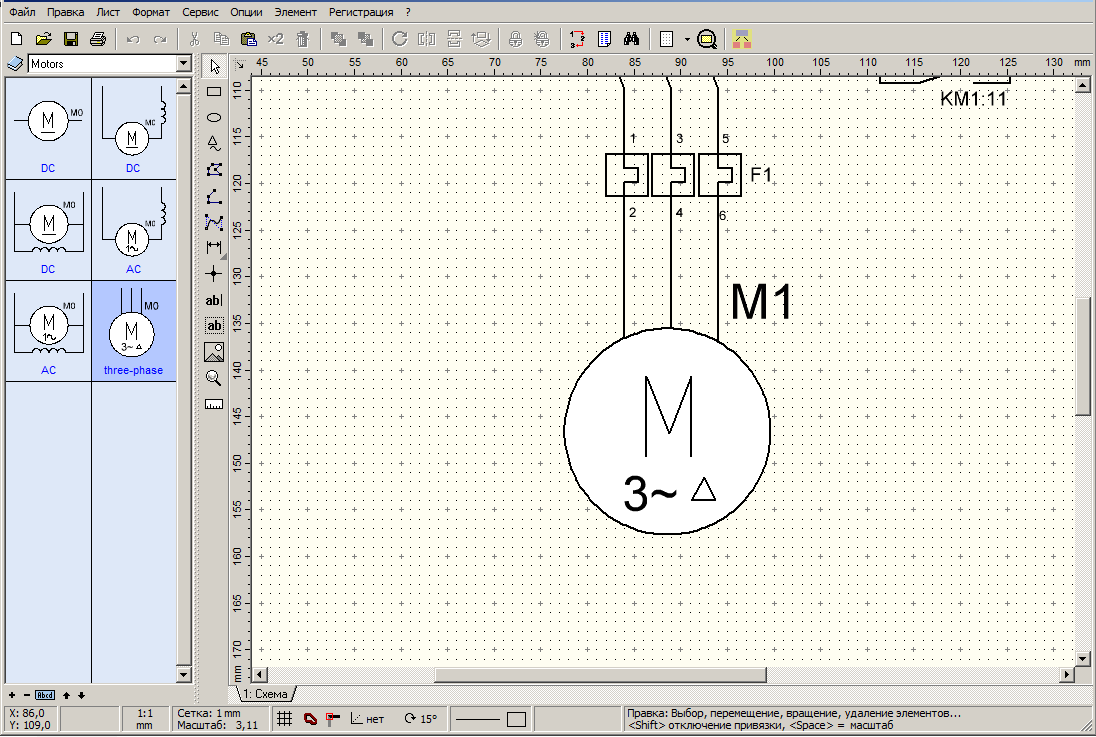
\includegraphics[width=0.7\linewidth]{./images/lab1/step1.png}
    \caption{\label{fig:lab1:step1} }
  \end{figure}
  \FloatBarrier

\item За допомогою інструменту ``Лінія'' створюємо з’єднання між елементами схеми
  (\ref{fig:lab1:step2}).
  \begin{figure}[!ht]
    \centering 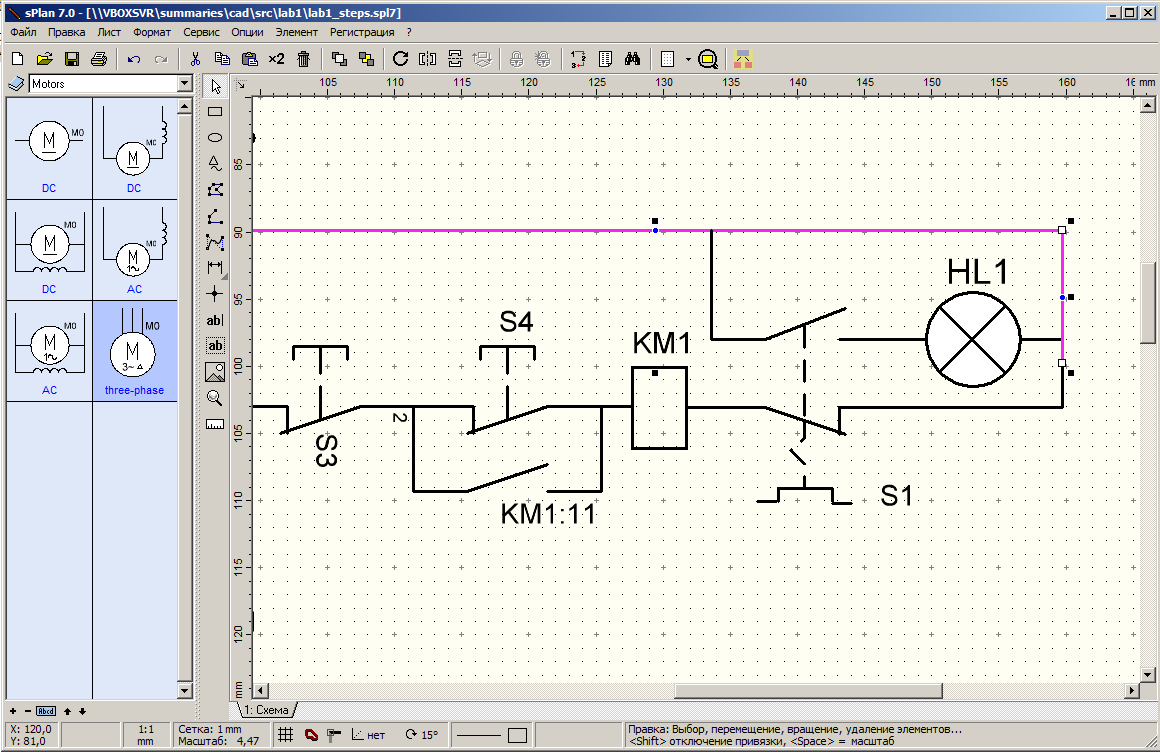
\includegraphics[width=0.7\linewidth]{./images/lab1/step2.png}
    \caption{Вікно налаштувань аркуша}
    \label{fig:lab1:step2} 
  \end{figure}
  \FloatBarrier

\item За допомогою інструменту ``Вузол'' задаємо вузли схеми.
  (\ref{fig:lab1:step2}). (\ref{fig:lab1:step3}).
  \begin{figure}[!ht]
    \centering 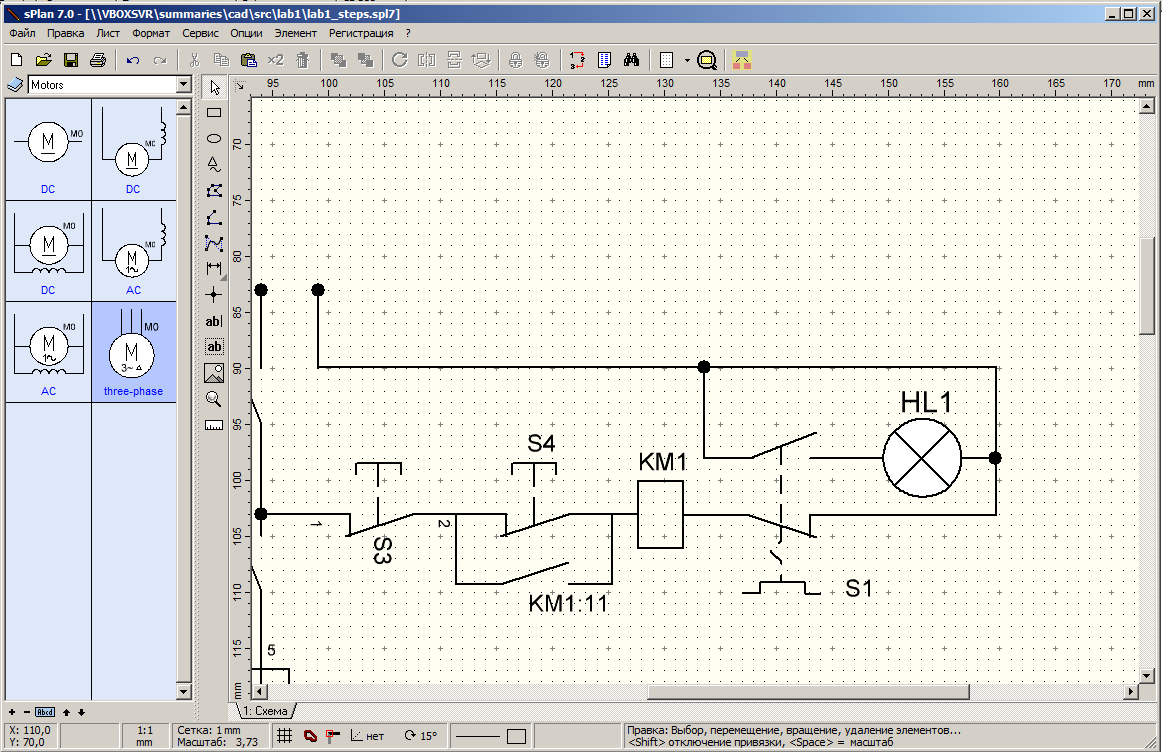
\includegraphics[width=0.7\linewidth]{./images/lab1/step3.png}
    \caption{Вікно налаштувань аркуша}
    \label{fig:lab1:step3} 
  \end{figure}
  \FloatBarrier

\item Необхідні текстові написи зажаємо інструментом ``Лінійний текст'' (\ref{fig:lab1:step4}).
  \begin{figure}[!ht]
    \centering 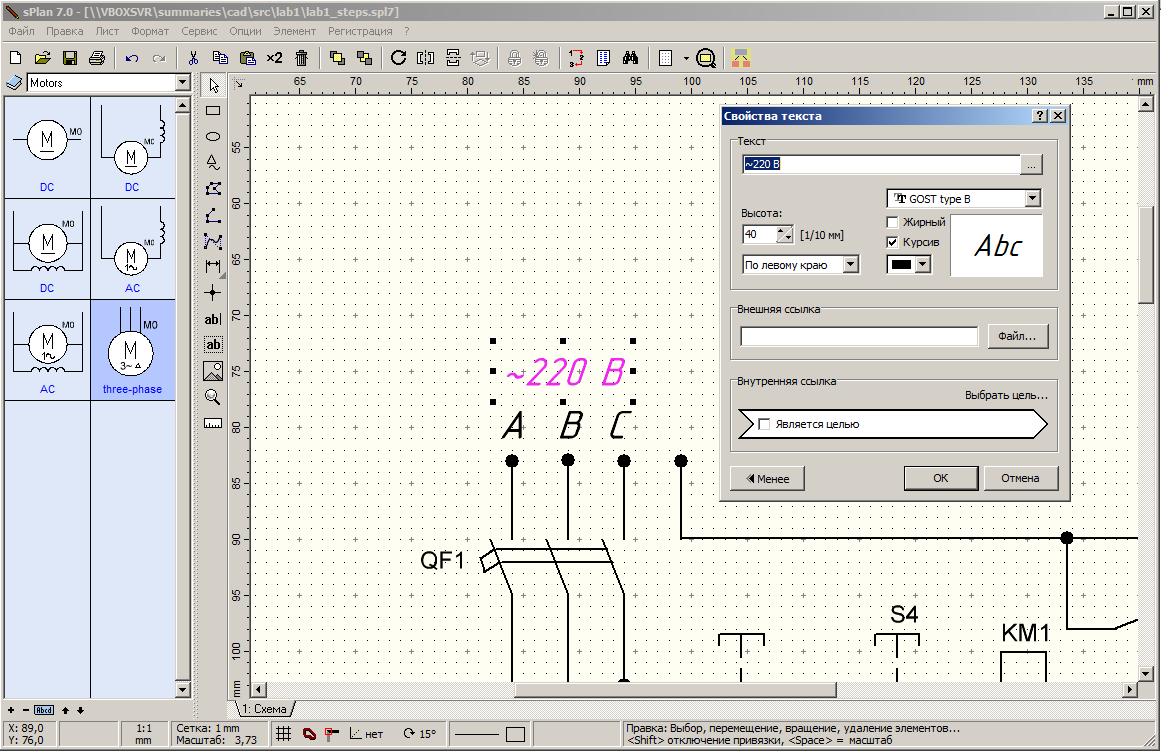
\includegraphics[width=0.7\linewidth]{./images/lab1/step4.png}
    \caption{Вікно налаштувань аркуша}
    \label{fig:lab1:step4} 
  \end{figure}
  \FloatBarrier
\end{enumerate}

Готовий кресленик навадений на сторінці \pageref{lab1:pdf:drawing}.
\newpage
\NoBorder
\label{lab1:pdf:drawing}
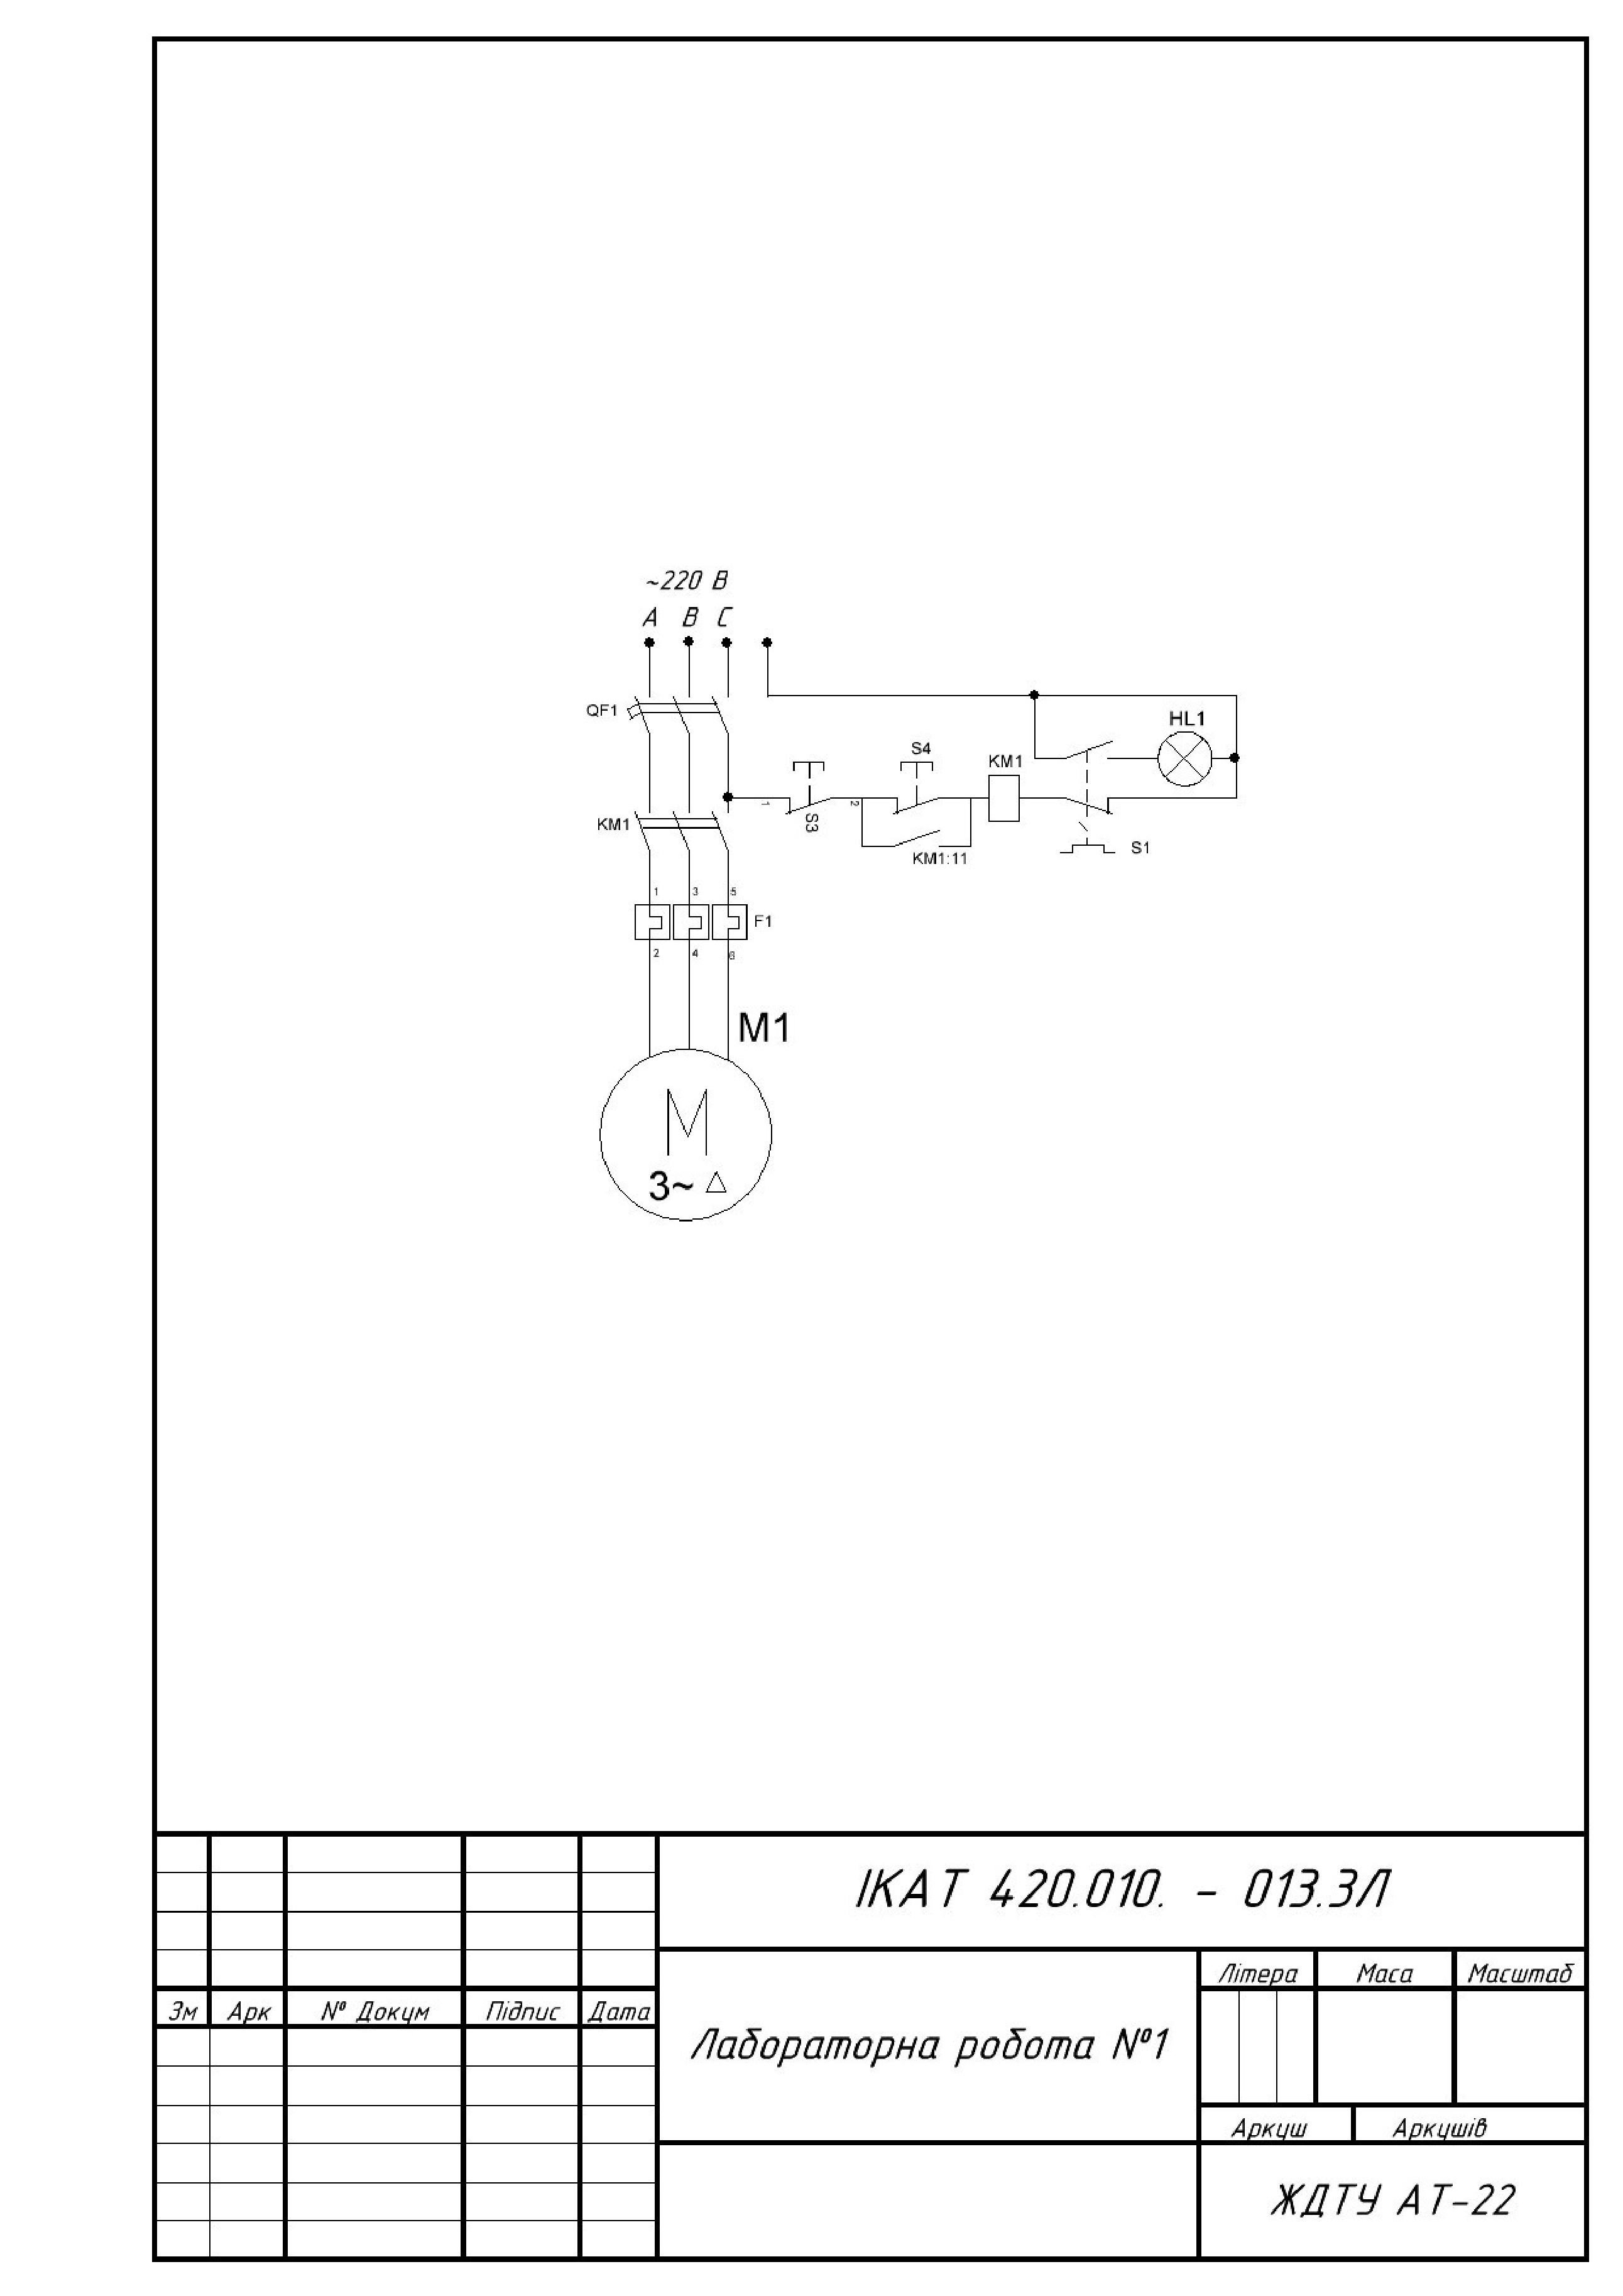
\includepdf{./src/lab1/drawing.pdf} \BorderText
\newpage

\BorderText

\section*{Висновки}

В межах даної лабораторної роботи було створено принципову схему САК з набору бібліотечних
елементів, та проведено ознайомлення з базовими приниципами та інструментами роботи в SPLAN.

За допомогою програми SPLAN можна відносно швидко проектувати принципові схеми та інші схематичні
зображення, створювати власні компоненти та шаблони, і використовувати його для робіт з виконання
схематичного зображення електронних схем.
